\documentclass{beamer}

\mode<presentation> {

    % The Beamer class comes with a number of default slide themes
    % which change the colors and layouts of slides. Below this is a list
    % of all the themes, uncomment each in turn to see what they look like.

    %\usetheme{default}
    %\usetheme{AnnArbor}
    %\usetheme{Antibes}
    %\usetheme{Bergen}
    %\usetheme{Berkeley}
    %\usetheme{Berlin}
    %\usetheme{Boadilla}
    %\usetheme{CambridgeUS}
    %\usetheme{Copenhagen}
    %\usetheme{Darmstadt}
    %\usetheme{Dresden}
    %\usetheme{Frankfurt}
    %\usetheme{Goettingen}
    %\usetheme{Hannover}
    %\usetheme{Ilmenau}
    %\usetheme{JuanLesPins}
    %\usetheme{Luebeck}
    \usetheme{Madrid}
    %\usetheme{Malmoe}
    %\usetheme{Marburg}
    %\usetheme{Montpellier}
    %\usetheme{PaloAlto}
    %\usetheme{Pittsburgh}
    %\usetheme{Rochester}
    %\usetheme{Singapore}
    %\usetheme{Szeged}
    %\usetheme{Warsaw}

    % As well as themes, the Beamer class has a number of color themes
    % for any slide theme. Uncomment each of these in turn to see how it
    % changes the colors of your current slide theme.

    %\usecolortheme{albatross}
    %\usecolortheme{beaver}
    %\usecolortheme{beetle}
    %\usecolortheme{crane}
    %\usecolortheme{dolphin}
    %\usecolortheme{dove}
    %\usecolortheme{fly}
    %\usecolortheme{lily}
    %\usecolortheme{orchid}
    %\usecolortheme{rose}
    %\usecolortheme{seagull}
    %\usecolortheme{seahorse}
    %\usecolortheme{whale}
%\usecolortheme{wolverine}

%\setbeamertemplate{footline} % To remove the footer line in all slides uncomment this line
%\setbeamertemplate{footline}[page number] % To replace the footer line in all slides with a simple slide count uncomment this line

%\setbeamertemplate{navigation symbols}{} % To remove the navigation symbols from the bottom of all slides uncomment this line
}

\usepackage{graphicx} % Allows including images
\usepackage{booktabs} % Allows the use of \toprule, \midrule and \bottomrule in tables


\usepackage{beamerthemeshadow}
\usepackage{latexsym,amsbsy,amsopn,amstext,xcolor,multicol,amsmath}
\usepackage{amssymb,graphicx,wrapfig,fancybox}
\usepackage{pgf,pgfarrows,pgfnodes,pgfautomata,pgfheaps,pgfshade}
\usepackage{booktabs}
\usepackage{subfloat}
\usepackage{}
\graphicspath{{figures/}}

%----------------------------------------------------------------------------------------
%	TITLE PAGE
%----------------------------------------------------------------------------------------

\title[Group Report]{Group Report on Recent Work}

\author{Ma Hsuning}
\institute[NKU]
{
    Physics of NKU\\
    \medskip
    \textit{maxn@ihep.ac.cn}
}
\date{\today}

%----------------------------------------------------------------------------------------
\begin{document}
%----------------------------------------------------------------------------------------
\frame{\titlepage}
%----------------------------------------------------------------------------------------

\begin{frame}
\frametitle{Overview}
\tableofcontents
\end{frame}
%----------------------------------------------------------------------------------------

\section{Motivation of recent work}
%----------------------------------------------------------------------------------------
\begin{frame}{Introduction}
\begin{block}{The process we are studying}
\begin{center}
$\psi\prime \rightarrow {\pi}^0 h_c$\\
        ${\pi}^0 \rightarrow \gamma \gamma$\\
        $h_c \rightarrow \gamma {\eta}_c$\\
        ${\eta}_c \rightarrow K_S^0 K \pi$\\
        $K_S^0 \rightarrow {\pi}^+ {\pi}^-$\\
        \end{center}
\end{block}
\bigskip
\begin{block}{The purpose of recent work}
Measure of the Branching ratio of the process $ {\eta}_c &\rightarrow& K_S^0 K \pi$
\end{block}
\end{frame}
%----------------------------------------------------------------------------------------

\begin{frame}{Method to do it}
\begin{itemize}
\item Fit ${\eta}_c$ signal with the recoil mass of $\gamma$ and ${\pi}^0$, requiring the reconstruction of ${\pi}^0$ and ${\gamma}_{\rm E1}$;
\bigskip
\item Fit ${\eta}_c$ with $K_S^0$, $K$ and $\pi$, requiring the reconstruction of $K_S^0$, $K$ and $\pi$;
\bigskip
\item The branching fraction will be acquired as the ratio of the two ${\eta}_c$ signal as
\begin{center}
\shadowbox{$Br({\eta}_c\rightarrow K_S^0 K \pi)=(\frac{N_{Obs1}}{N_{Obs2}}\cdot \frac{{\epsilon}_2}{{\epsilon}_1} \cdot \frac{1}{Br({\pi}^0 \rightarrow \gamma \gamma) \cdot Br(K_S^0 \rightarrow {\pi}^+ {\pi}^-)})^{\frac{1}{2}}$}
\end{center}
\end{itemize}
\end{frame}
%----------------------------------------------------------------------------------------

\section{Event Selection}
\subsection{Reconstruction of $K_S^0$ $K$ and $\pi$}
%----------------------------------------------------------------------------------------

\begin{frame}{}
\begin{block}{Selection of $\gamma$ and ${\pi}^0$}
\begin{itemize}
\item $E_{\gamma}>25 MeV$,$|\cos\theta|<0.8$ ( barrel region )
\item $E_{\gamma}>50 MeV$,$0.86<|\cos\theta|<0.92$ ( end-cap region )
\item $450MeV < E({\gamma}_{{\rm E1}}) < 550MeV$
\item $|M_{\gamma \gamma}-m_{{\pi}^0}| < 15 MeV/c^2$
\end{itemize}
\end{block}
\begin{block}{Selection of charged tracks}
\begin{itemize}
\item $ | \cos\theta |<0.93$
\item $|R_{z}|<10cm$,$R_{xy}<1cm$ for charged tracks from ${\eta}_c$
\item The Track is the particle type with the highest confidence level.
\item $ |M_{\pi \pi} - m_{K_S^0} | < 20 MeV/c^2$ ( Reconstruction $K_S^0 \rightarrow {\pi}^+ {\pi}^-$ )
\end{itemize}
\end{block}
\shadowbox{We accept the one with the smallest ${\chi}^2={\chi}_{4C}^2+{\chi}_{1C}^2+{\chi}_{pid}^2+{\chi}_{vertex}^2$.}
\end{frame}
%----------------------------------------------------------------------------------------
\subsection{Reconstruction of ${\gamma}_{\rm E1}$ and ${\pi}^0$}
%----------------------------------------------------------------------------------------

\begin{frame}{}
\shadowbox{This is a different process}
\begin{block}{Selection of good photons}
\begin{itemize}
\item $E_{\gamma}>25 MeV$,$|\cos\theta|<0.8$ ( barrel region )
\item $E_{\gamma}>50 MeV$,$0.86<|\cos\theta|<0.92$ ( end-cap region )
\end{itemize}
\end{block}
\begin{block}{Selection of ${\rm E1}_{\gamma}$ and ${\pi}^0$}
\begin{itemize}
\item $450MeV < E({\gamma}_{{\rm E1}}) < 550MeV$
\item $|M_{\gamma \gamma}-m_{{\pi}^0}| < 15 MeV/c^2$
\end{itemize}
\end{block}
\begin{block}{Event selected}
The one with the smallest ${\chi}^2 = {\chi}_{1C}^2 + {(\frac{m_{recoil}({\pi}^0)-m_{h_c}}{{\sigma}_{h_c}})}^2 + (\frac{m_{recoil}(\gamma {\pi}^0)-m_{{\eta}_c}}{{\sigma}_{{\eta}_c}})^2$ will do.
\end{block}
\end{frame}
%----------------------------------------------------------------------------------------

\section{signal MC Results}
\subsection{Results of reconstruction of $K_S^0$ $K$ and $\pi$}
%----------------------------------------------------------------------------------------
\begin{frame}{Energy of ${\gamma}_{\rm E1}$}
\begin{center}
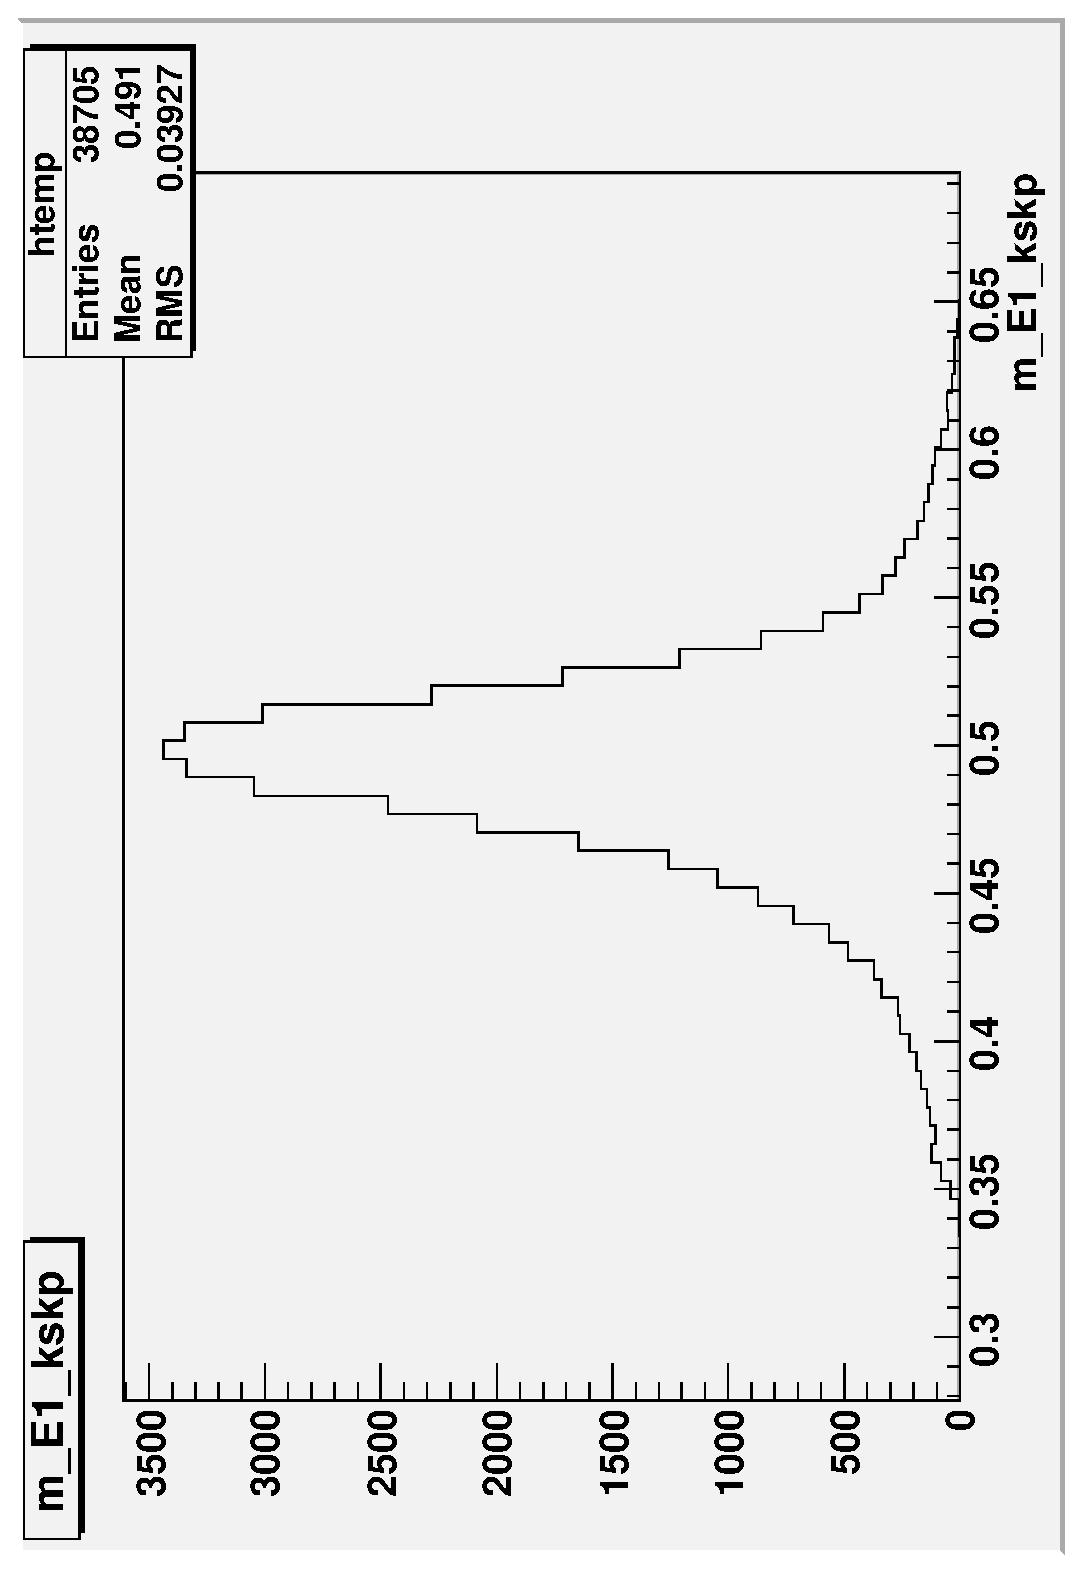
\includegraphics[width=0.5\textwidth,angle=270]{figures/m_E1_kskp.eps}
\end{center}
\end{frame}

%----------------------------------------------------------------------------------------
\begin{frame}{Invariant mass of $h_c$}
\begin{center}
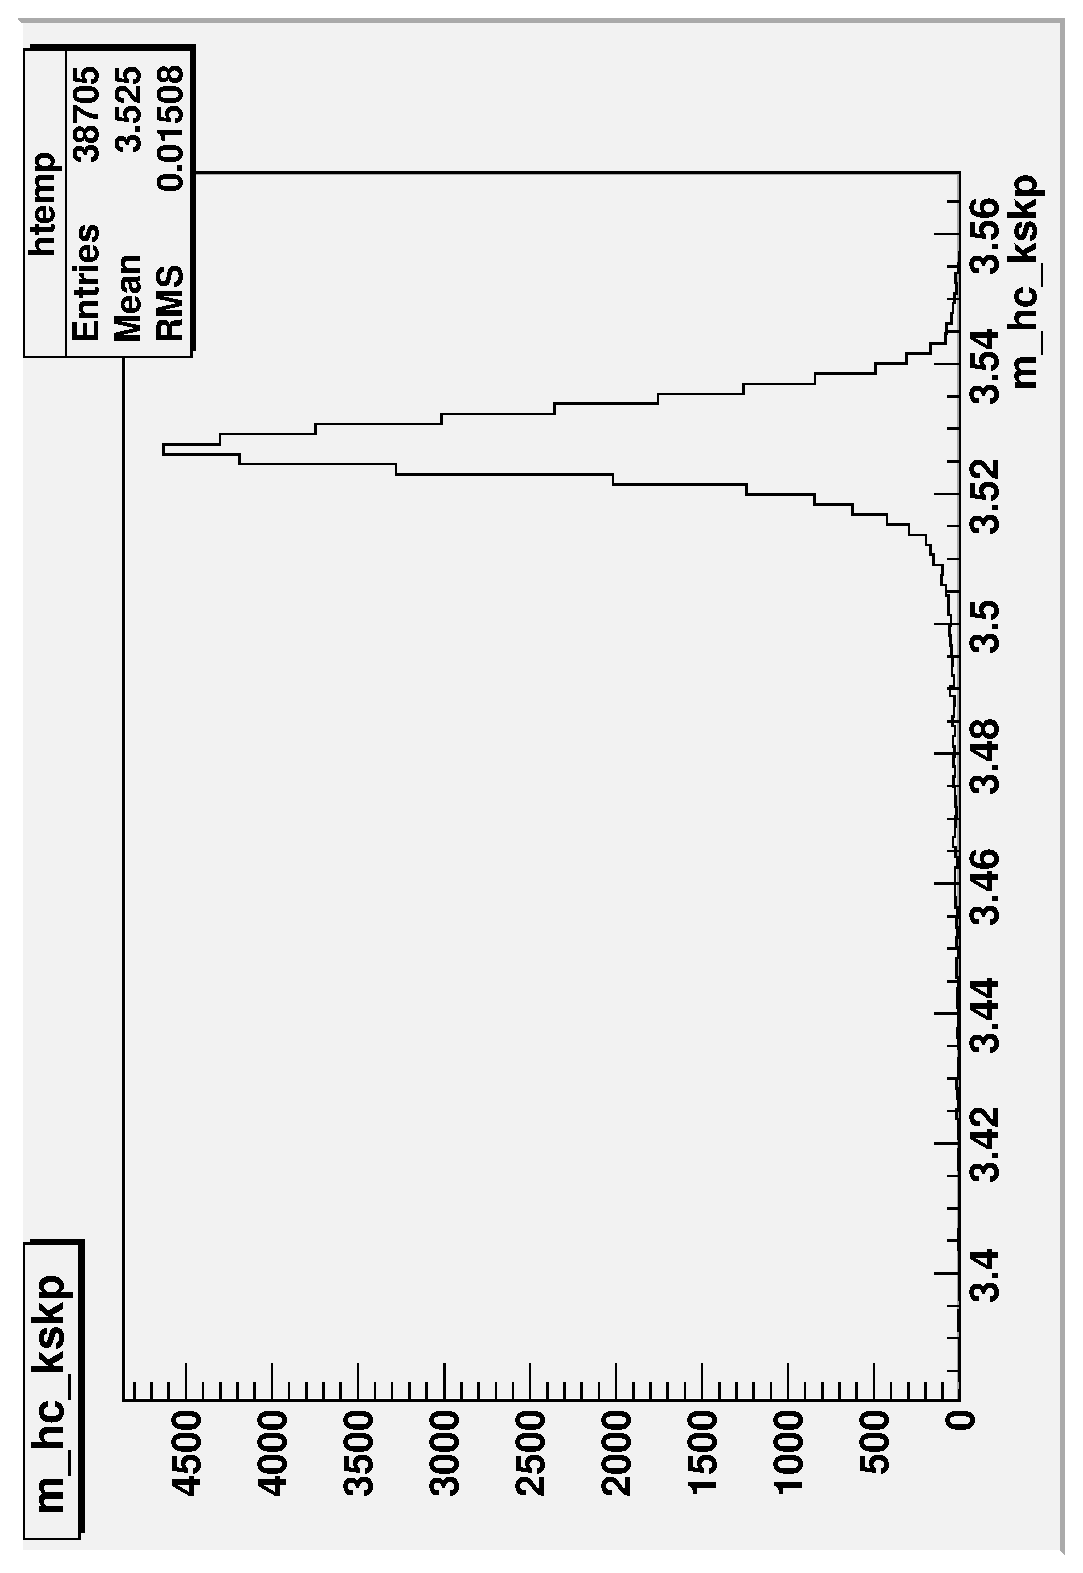
\includegraphics[width=0.5\textwidth,angle=270]{figures/m_hc_kskp.eps}
\end{center}
\end{frame}
%----------------------------------------------------------------------------------------
\begin{frame}{Invariant mass of ${\eta}_c$}
\begin{center}
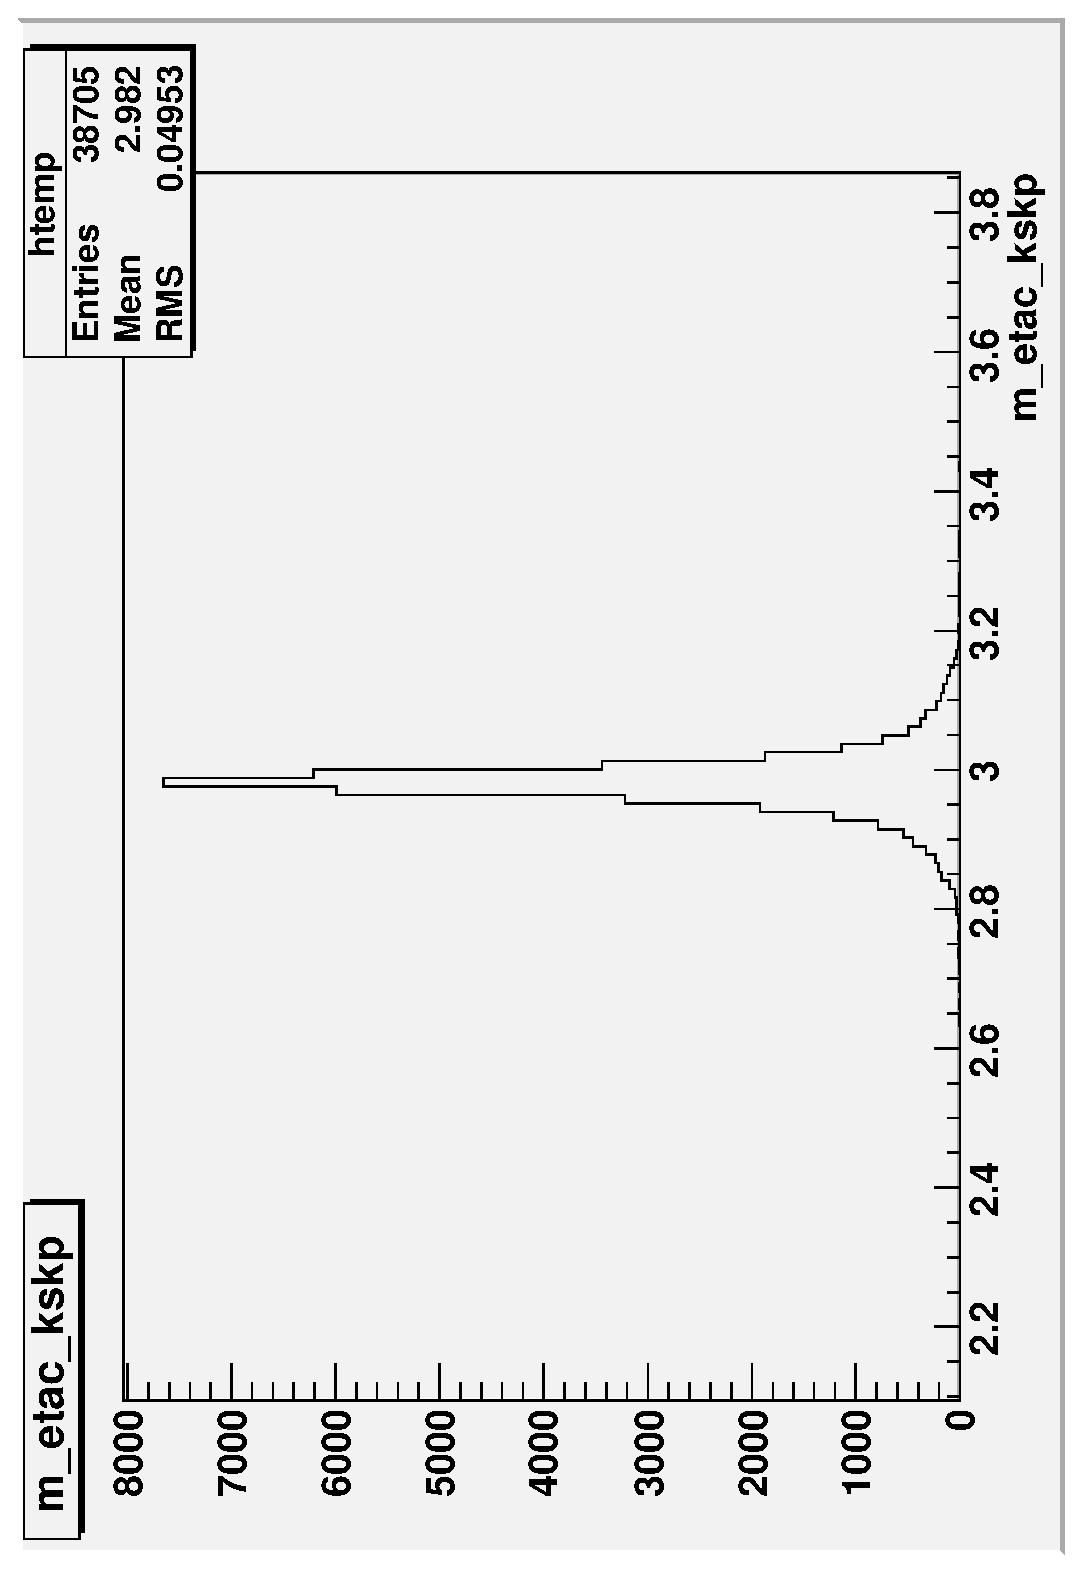
\includegraphics[width=0.5\textwidth,angle=270]{figures/m_etac_kskp.eps}
\end{center}
\end{frame}
%----------------------------------------------------------------------------------------

\subsection{Results of reconstruction of ${\gamma}_{\rm E1}$ and ${\pi}^0$}
%----------------------------------------------------------------------------------------
\begin{frame}{Energy of ${\gamma}_{\rm E1}$}
\begin{center}
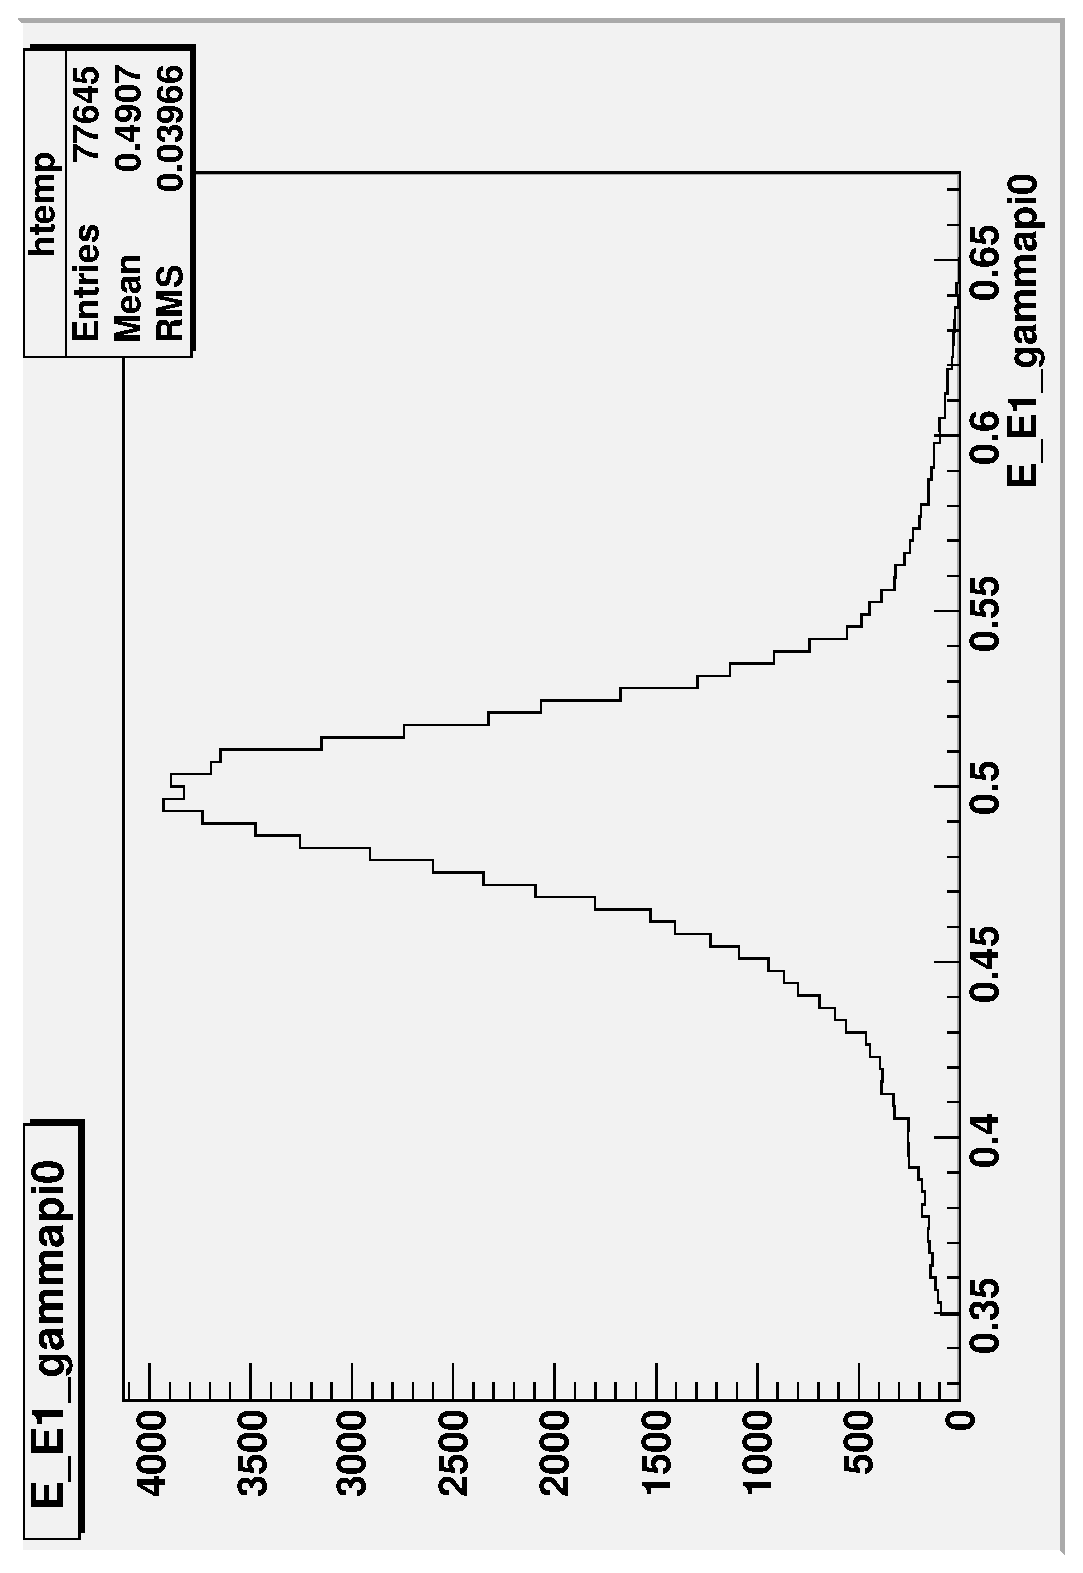
\includegraphics[width=0.5\textwidth,angle=270]{figures/E_E1_gammapi0.eps}
\end{center}
\end{frame}
%----------------------------------------------------------------------------------------
\begin{frame}{Recoil mass of ${\pi}^0$}
\begin{center}
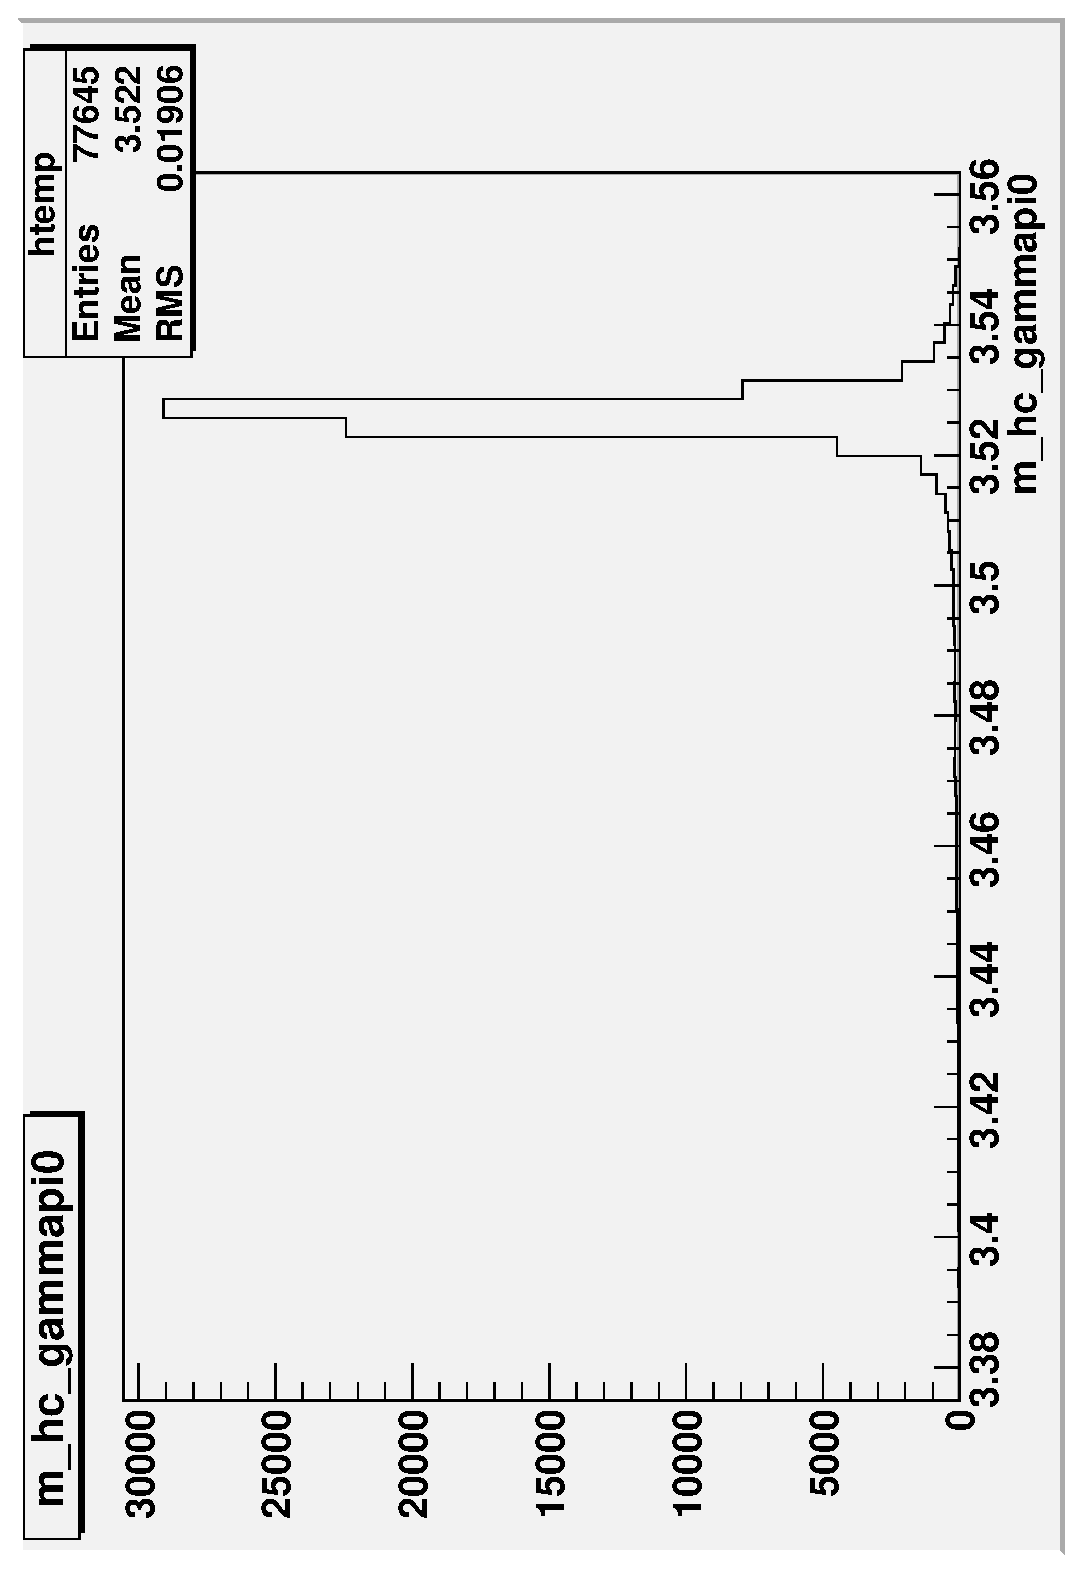
\includegraphics[width=0.5\textwidth,angle=270]{figures/m_hc_gammapi0.eps}
\end{center}
\end{frame}
%----------------------------------------------------------------------------------------
\begin{frame}{Recoil mass of ${\gamma}_{\rm E1}$ and ${\pi}^0$}\label{fig5}
\begin{center}
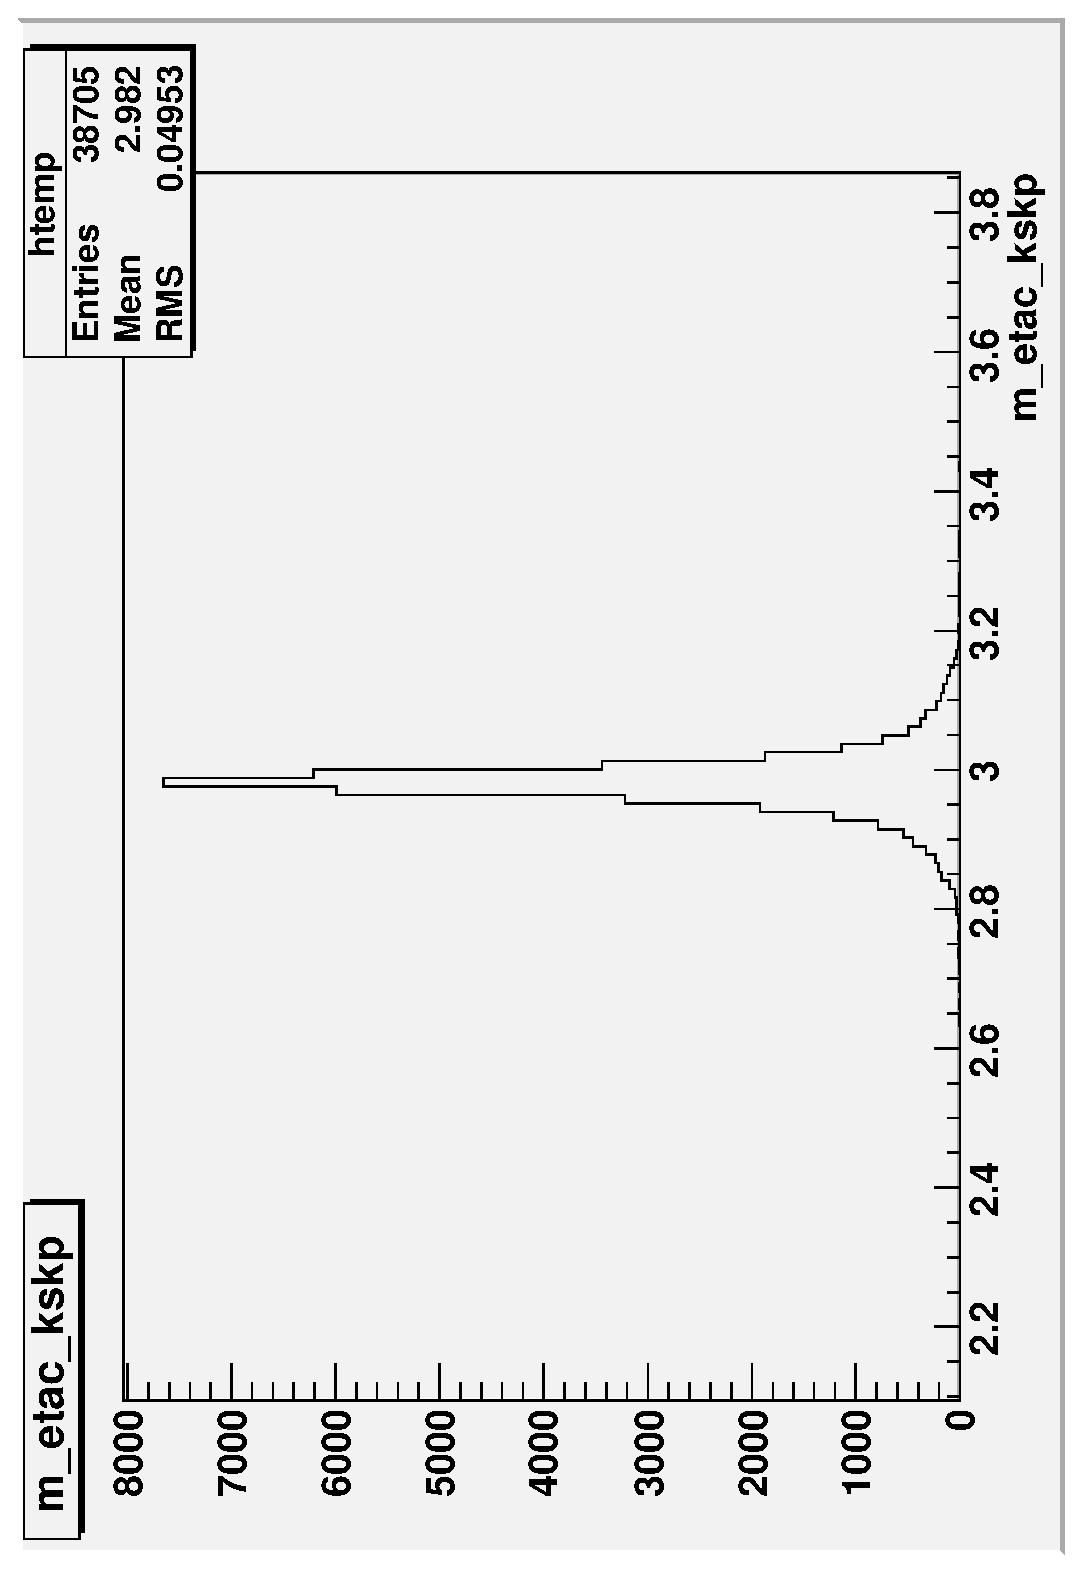
\includegraphics[width=0.5\textwidth,angle=270]{figures/m_etac_kskp.eps}
\end{center}
\end{frame}
%----------------------------------------------------------------------------------------

\section{Work to be done}
%----------------------------------------------------------------------------------------
\begin{frame}{Time table}
\begin{itemize}
\item Debug the analysis program in less than one week
\item Optimize the selection in 2-3 weeks
\item Analyze the background in 2-3 weeks
\item Fit the signal and get the preliminary results in 2-3 weeks
\item Deal with the system error in about 3 months
\end{itemize}
\end{frame}

%----------------------------------------------------------------------------------------
\end{document}
